\chapter{Introducción y descripción de Broadsea} \label{cap:01Introduccion}

\section{Introducción al Manual} \label{cap:01.1IntroManual}

Este manual ha sido redactado entre Febrero y Marzo de 2024 con motivo de complementar como anexo al Trabajo de Fin de Grado \textit{Extrayendo conocimiento a partir de análisis clínico de datos CDM usando la herramienta Atlas}
de la misma autora, Maria del Valle Alonso de Caso Ortiz, y sobre la misma herramienta, ATLAS.

%\subsubsection{Necesidad que satisface este anexo.}

Dicha herramienta, por ser de código abierto, presenta multitud de información esparcida y repartida de forma pseudo-ordenada entre repositorios de github y foros de la comunidad OHDSI pero no se encontró ningún manual que recopilase toda la información de instalación y despliegue en un único sitio. Por tanto, a la hora de instalar y desplegar la herramienta, con objeto de su utilización en el TFG, se encontraron numerosas dificultades para encontrar procedimientos concretos y guiados.

Si bien había mucha información en la red sobre cómo realizar diferentes tipos de instalaciones, en la mayoría de los casos presentaban (i) información poco específica con asumición de conocimientos previos no mencionados (ii) información dificilmente accesible por presentarse en diferentes localizaciones en la red (iii) poca información de resolución de problemas, mayoritariamente presente en foros con problemas específicos de los cuales había que sacar conocimientos generales, entre otros.  

De esta dificultad experimentada por la alumna fue de donde se originó la idea de redactar este anexo, para aportar a la comunidad OHDSI y a cualquier usuario que pretendiese utilizar la herramienta, una guía detallada paso a paso que facilitase y agrupase toda la información necesaria y la resolución de posibles confictos durante la instalación, despliegue y configuración de ATLAS en el entorno de Broadsea. 

%\subsubsection{Contexto de implementación de la herramienta.}

No obstante, no es obviable el fin último del manual de acompañar al Trabajo Fin de Grado, desarrollado en compañía del grupo de Innovación Tecnológica del Hospital Universitario Virgen del Rocío, por lo que, frente a la multitud de posibilidades de configuración de distintos aspectos de la herramienta, aunque el manual presenta todos ellos, en númerosas ocasiones solo se centra en los procedimientos que aplican a las necesidades del TFG y del departamento del Hospital.

Es decir, el manual se desarrolla en un contexto de implementación de ATLAS Broadsea bajo los requisitos de una organización pública, el HUVR, con fines de ayudar y dar soporte a las investigaciones realizadas en el mismo, y bajo la supervisión continua de Da. Silvia Rodríguez Mejías y Dr. Carlos Parra Calderón.

%\subsubsection{Información adicional.}

Toda la información que se ha generado durante y tras la redacción de este documento, y del TFG, se encuentra en un repositorio de github público, para permitir el acceso de cualquier usuario a comprobar archivos generados de variables, logs, scripts de código, etcétera. Para mayor información consultar el link del repositorio \cite{vallealonsodc}.

\section{Descripción de Broadsea} \label{cap:01.2descripBroadsea}

%ATLAS es una plataforma de análisis de datos de ciencia abierta perteneciente a la red OHDSI para facilitar el intercambio de estructuras de análisis entre organizaciones pertenecientes a esta misma red. ATLAS se sostiene sobre el modelo de datos común de OMOP (CDM) que es el objeto de unión de todos los estudios OHDSI, la normalización de las bases de datos a este estándar clínico.

%Para facilitar la implementación de ATLAS, OHDSI propone diversas alternativas dependiendo de las necesidades de la organización interesada. En este manual se presenta la implementación, instalación, despliegue y configuración a través de Broadsea.

Con objeto de la implementación de ATLAS satisfaciendo el marco del desarrollo del Trabajo Fin de Grado y el entorno de investigación del hospital (véase \ref{cap:01.1IntroManual}), se decide adoptar Broadsea como la alternativa más sencilla para implementar, desplegar y configurar la herramienta.

Broadsea es un proyecto basado en Docker que permite desplegar un entorno de herramientas, configuraciones y dependencias OHDSI de la manera más sencilla hasta el momento. De hecho, la misma organización la presenta, textualmente, como \textit{''la forma más sencilla de instalar (y actualizar) las herramientas OHDSI"} \cite{Broadsea3PDF}. 

Lo que comenzó, en su primera versión, como un simple contenedor que albergase imágenes de la WebAPI de ATLAS y RStudio \cite{Broadsea3PPTX} ha evolucionado hasta la tercera versión en la que Broadsea alberga la mayoría de herramientas OHDSI, creando un entorno virtual de desarrollo muy completo.

\begin{figure}[H]
    \centering
    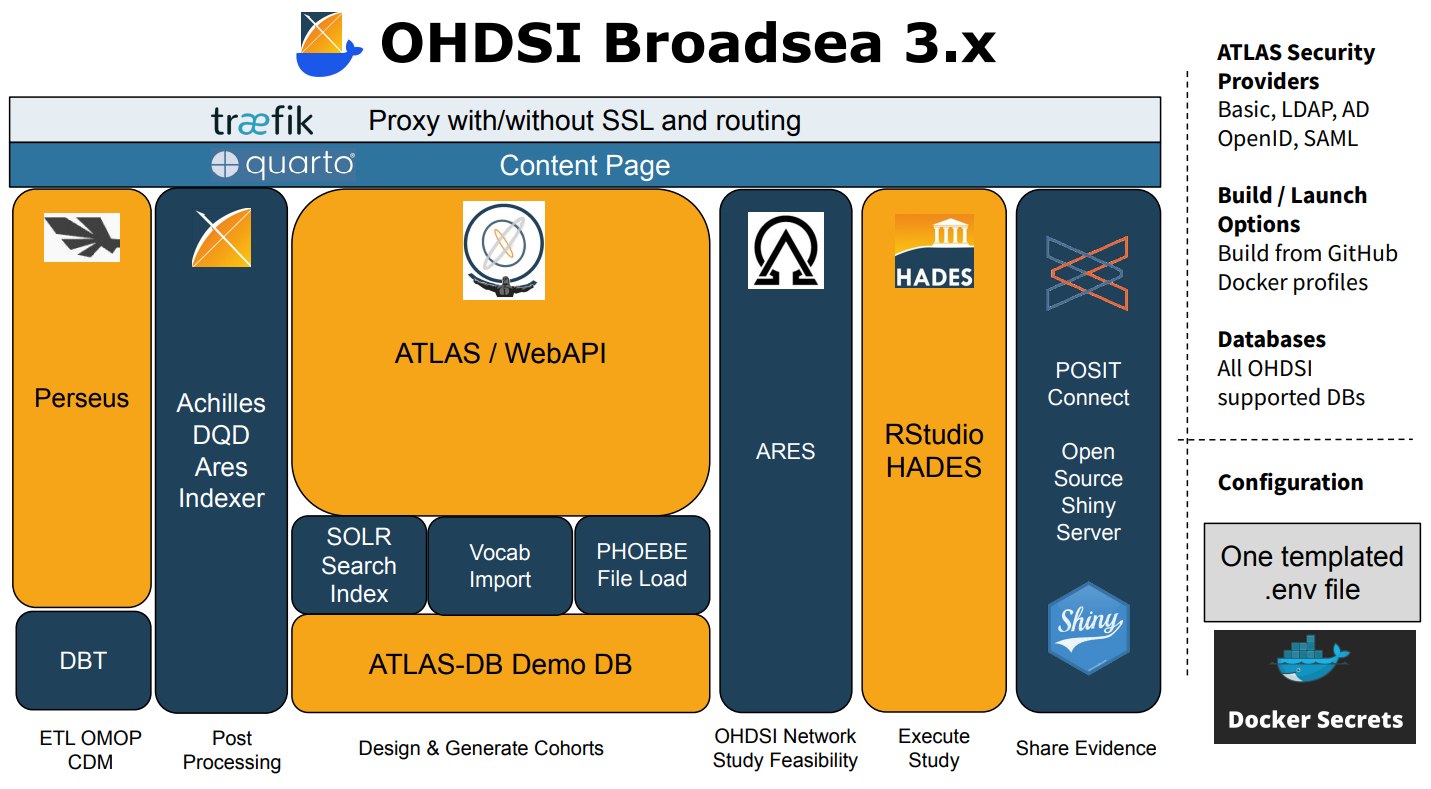
\includegraphics[width=0.90\textwidth]{figures/OHDSIBroadsea3.0.png}
    \caption{Vista general de todos los componentes de Broadsea. Extraída de \cite{Broadsea3PPTX}.}
    \label{fig:OHDSIBroadsea3.0}
\end{figure}

Este manual tan solo se centra en la instalación, despliegue y configuración de ATLAS (y la WebAPI) pero las posibilidades de utilización de otras herramientas son múltiples. A partir de este momento se le denomina ATLAS Broadsea a la herramienta ATLAS que ofrece el entorno Broadsea.


\section{Entorno Docker de Broadsea} \label{cap:01.3Docker}

En la práctica, el entorno de Broadsea se despliega como un multicontenedor Docker con varios perfiles preconfigurados que permiten ir añadiendo o eliminando configuraciones avanzadas del entorno. La descripción general del multicontenedor y sus perfiles se encuentra online en el repositorio de github de Broadsea \cite{githubBroadsea}.  

\subsubsection{Archivos de orquestación de contenedores}

Existen dos archivos clave en el repositorio que orquestan y coordinan los parámetros de configuración del multicontenedor: el \code{docker-compose.yml} y el archivo \code{.env}.

\begin{enumerate}

    \item El \code{docker-compose.yml} o simplemente \code{docker-compose} es el archivo docker que construye el entorno Broadsea, en él se describen los diferentes perfiles y sus parámetros y configuraciones más importantes. Es decir, cuando se construye el multicontenedor o se pretende ejecutar alguno de sus perfiles se llama a este archivo, que es el que contiene toda la información Docker relevante (véase \ref{cap:02Deployment}).

    Este archivo, por la relevancia que tiene en cuanto a la construcción del entorno Docker, no debería ser modificado, aunque puede ser de gran interés para comprobar la configuración o incluso la relación entre los diferentes perfiles, contenedores o volúmenes. A continuación se muestra una captura de pantalla a modo de ejemplo del archivo, abierto en Visual Studio Code.

\begin{figure}[H]
    \centering
    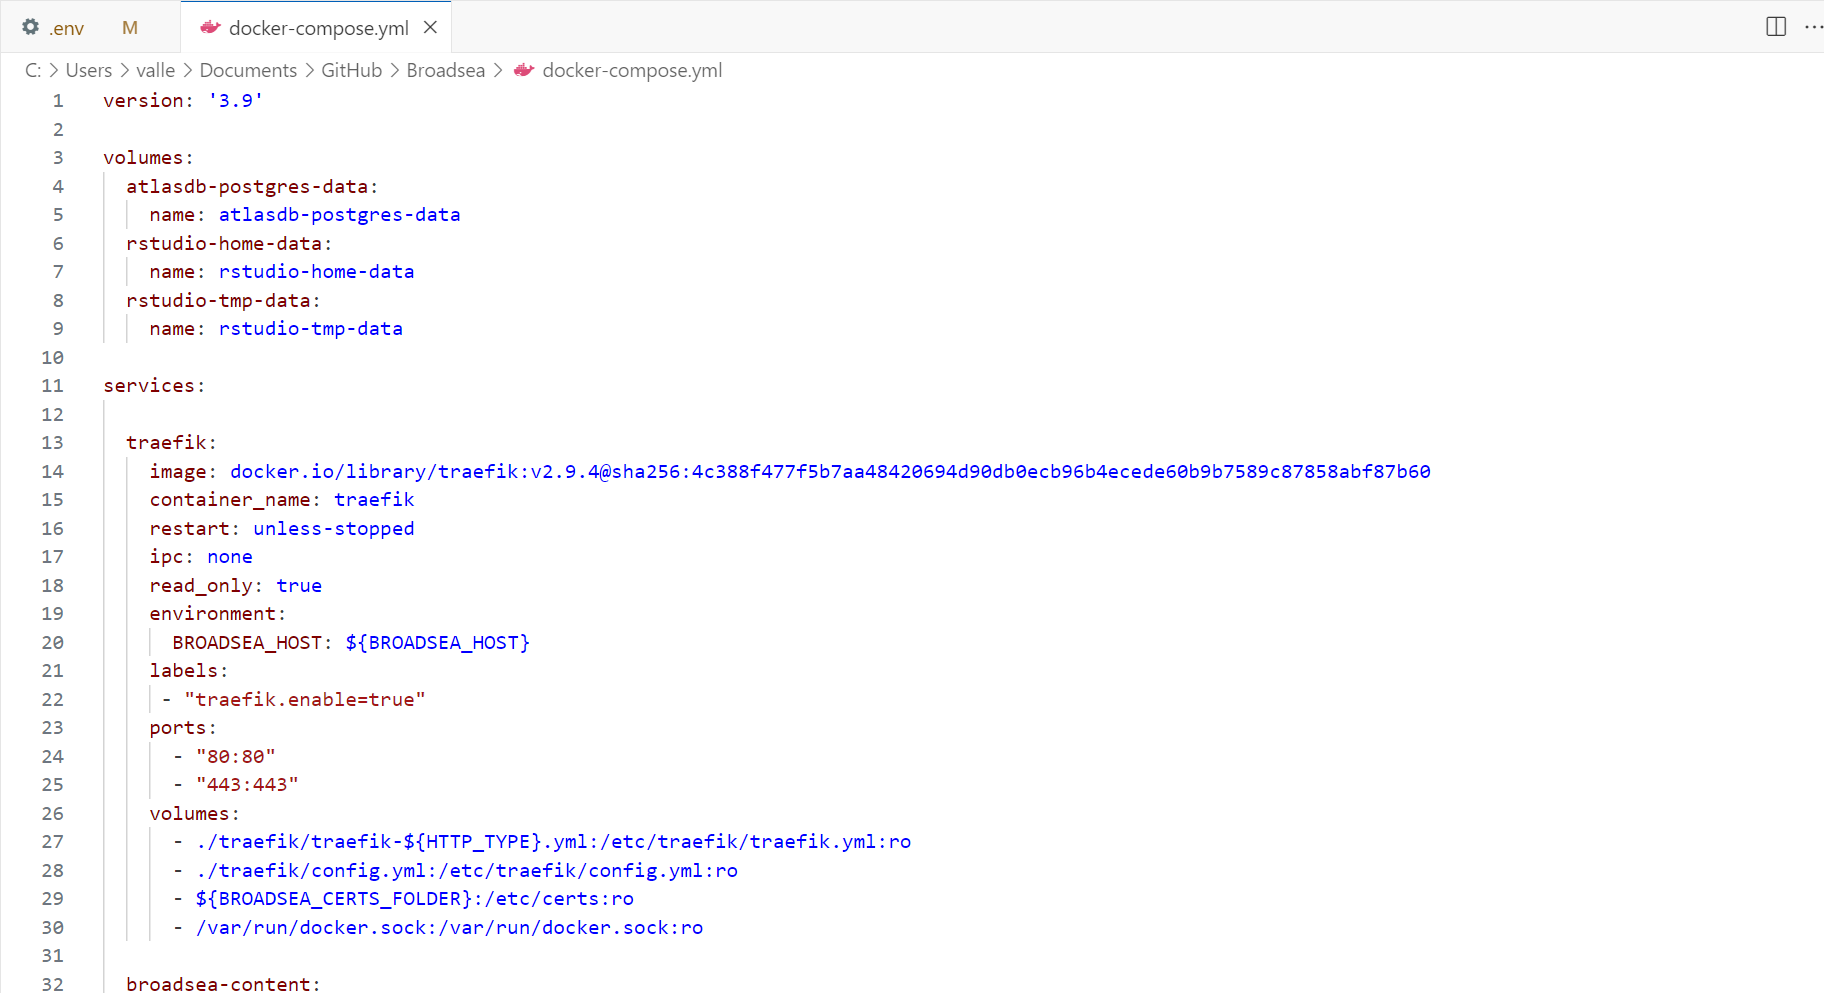
\includegraphics[width=0.90\textwidth]{figures/dockerCompose.png}
    \caption{Captura de pantalla de las primeras líneas del \code{docker-compose.yml}}
    \label{fig:dockerCompose}
\end{figure}

    \item El archivo \code{.env} es el archivo que contiene todas las configuraciones y parámetros modificables o customizables del entorno de Broadsea.

    A diferencia del \code{docker-compose}, la modificación de parámetros de este archivo será requerida en numerosas ocasiones para activar o desactivar ciertos parámetros o modificar algunas configuraciones del entorno. No obstante, también puede ser de gran interés para comprobar información relevante sobre los parámetros de funcionamiento del multicontenedor. A continuación se muestra una captura de pantalla a modo de ejemplo del archivo, abierto en Visual Studio Code.

\begin{figure}[H]
    \centering
    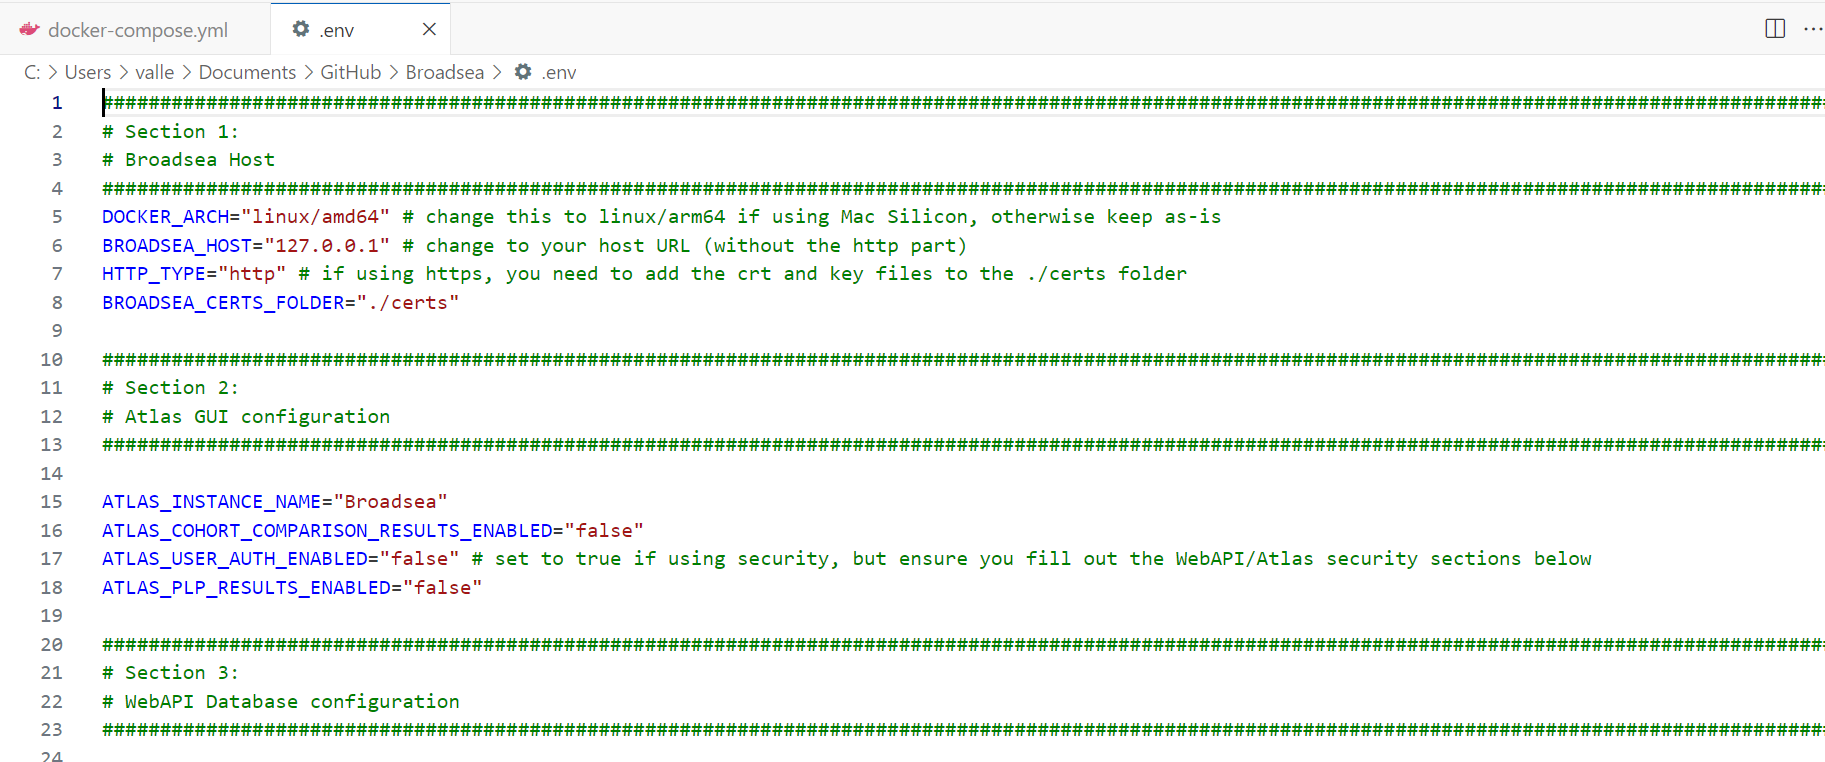
\includegraphics[width=0.90\textwidth]{figures/envFile.png}
    \caption{Captura de pantalla de las primeras líneas del archivo \code{.env}.}
    \label{fig:envFile}    
\end{figure}

    Como se puede apreciar en la imagen, este archivo está organizado en diferentes secciones, y presenta numerosos comentarios para facilitar al usuario la comprensión de los parámetros que debe modificar para establecer las configuraciones avanzadas del entorno.
    
    Hay doce secciones distintas: (1) Contiene la configuración del servidor donde se aloja Broadsea, (2) contiene la configuración de la interfaz gráfica de ATLAS, (3) contiene la configuración de la base de datos de ATLAS, (4) contiene la configuración del protocolo de seguridad de ATLAS, (5) contiene la configuración del protocolo de seguridad de la WebAPI, (6) contiene la configuración de ATLAS y la WebAPI mediante Github, (7) contiene la configuración del vocabualario de Apache Solr,  (8) contiene la configuración de identificación en HADES, (9) contiene la configuración del vocabulario de Postgres, (10) contiene la configuración de PHOEBE, (11) contiene la configuración de ARES, (12) contiene la configuración de la página inicial de Broadsea.
        
\end{enumerate}

\subsubsection{Perfiles de configuración}

En cuanto a los perfiles, a la hora de desplegar por primera vez el multicontenedor (véase \ref{cap:02Despliegue}), se ejecuta el perfil \code{default}, es decir, por defecto, que instala seis contenedores que proveen las herramientas básicas de Broadsea:  la WebAPI, el traefik, ATLAS y HADES y la base de datos de ATLAS (véase Figura \ref{fig:OHDSIBroadsea3.0}). A partir de este momento, el resto de configuraciones adicionales se realizan a través de los once perfiles restantes, descritos en el \code{docker-compose} y en el repositorio \cite{githubBroadsea}

\subsubsection{Volúmenes de almacenamiento de datos}

Además de los contenedores, Broadsea implementa tres volúmenes por defecto: un volumen para albergar la base de datos de ATLAS (\code{atlasdb-postgres-data}) y dos para la información de HADES (\code{rstudio-home-data} y \code{rstudio-tmp-data}). 

Los volúmenes de docker proporcionan una forma de persistir datos más allá del ciclo de vida de un contenedor y permiten compartir datos entre contenedores o entre un contenedor y el host. La información sobre los volúmenes y las relaciones que guardan con los contenedores se encuentra en el \code{docker-compose}. Una vez que se despliegue Broadsea en el equipo, hay dos formas de comprobar qué volúmenes se están ejecutando: (i) a través de la interfaz gráfica de Docker Desktop - Figura \ref{fig:dockerVolumes} (ii) a través del \code{cmd} - Figura \ref{fig:dockerVolumesCDM}.

\begin{figure}[H]
    \centering
    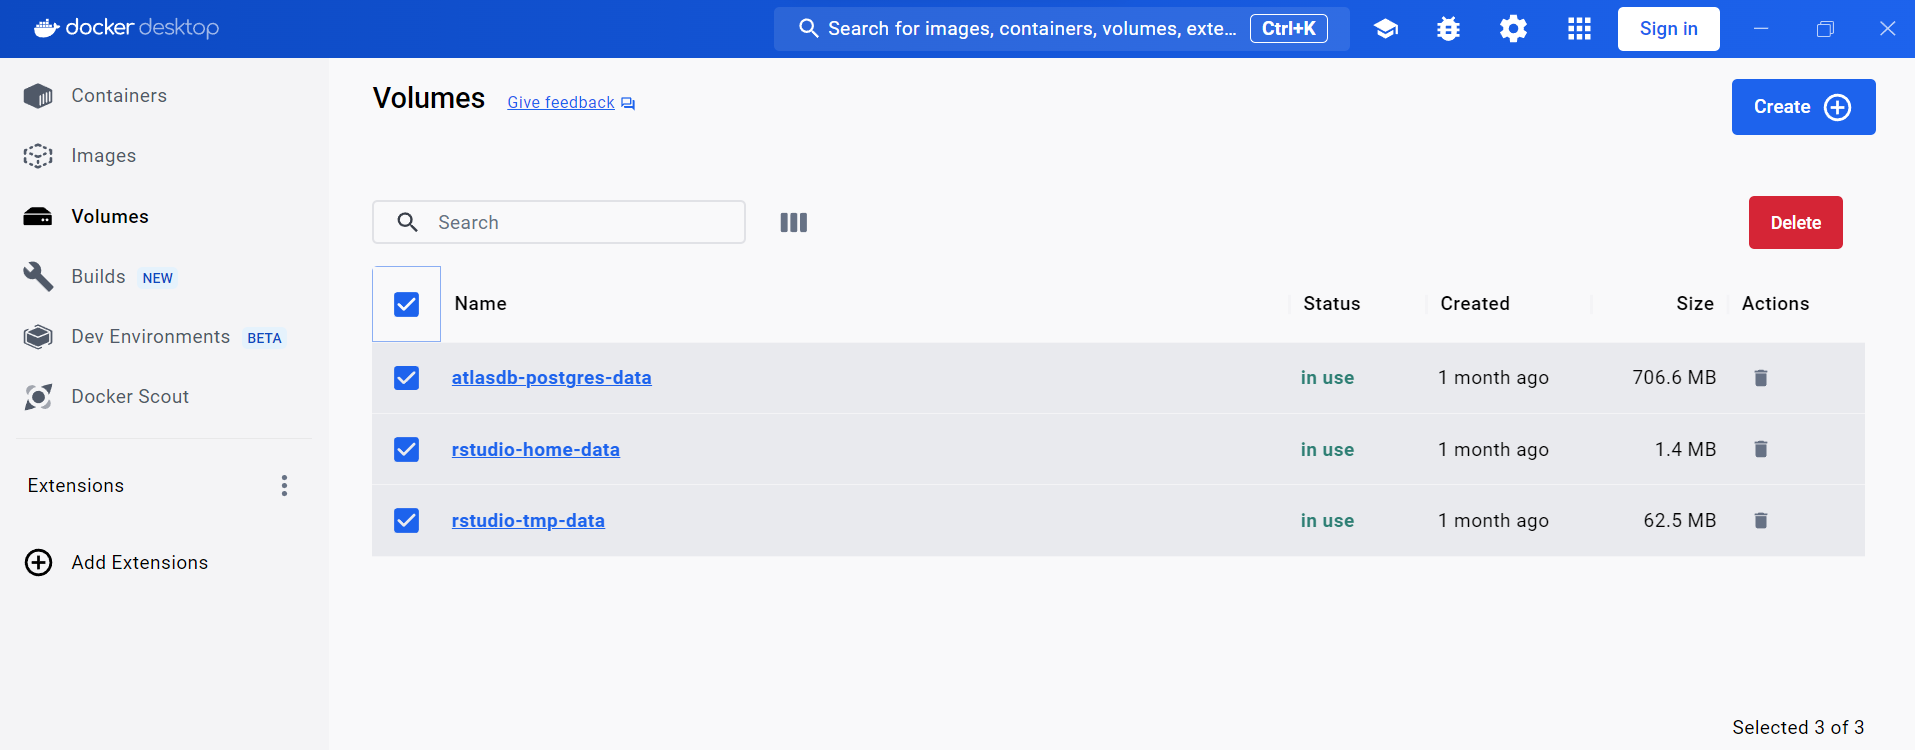
\includegraphics[width=0.90\textwidth]{figures/dockerVolumes.png}
     \caption{Captura de pantalla del panel \code{volumes} de Docker Desktop}
    \label{fig:dockerVolumes}
\end{figure}

\begin{figure}[H]
    \centering
    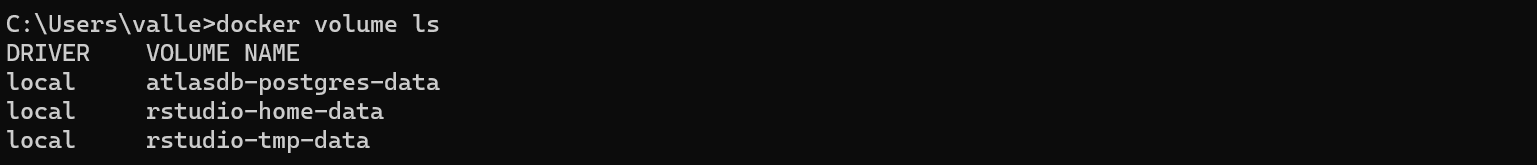
\includegraphics[width=0.90\textwidth]{figures/dockerVolumesCDM.png}
     \caption{Captura de pantalla del comando \code{docker volume ls} en el \code{cmd}}
    \label{fig:dockerVolumesCDM}
\end{figure}

El volumen  (\code{atlasdb-postgres-data}) será de especial interés durante la configuración de la base de datos de ATLAS (véase \ref{cap:03ConexLocal}).

\section{Entorno PostgreSQL de Broadsea}\label{01.4Postgre}

La configuración y relación entre las diferentes bases de datos que interaccionen con Broadsea se realiza a través de la WebAPI de ATLAS, que se aloja en un servidor de base de datos PostgreSQL. La documentación sobre la WebAPI es muy extensa y se encuentra en un repositorio principal de github \cite{githubWebAPI} que se divide en diferentes secciones de interés.

\subsection{La WebAPI}

\subsubsection{Estructura teórica}

En la wiki del repositorio \cite{githubWebAPIwiki} se da información más detallada sobre la webAPI y se define como ''una aplicación basada en Java diseñada para proporcionar un conjunto de servicios web RESTful para interactuar con una o más bases de datos'' y se caracteriza según la siguiente estructura:

\begin{figure}[H]
    \centering
    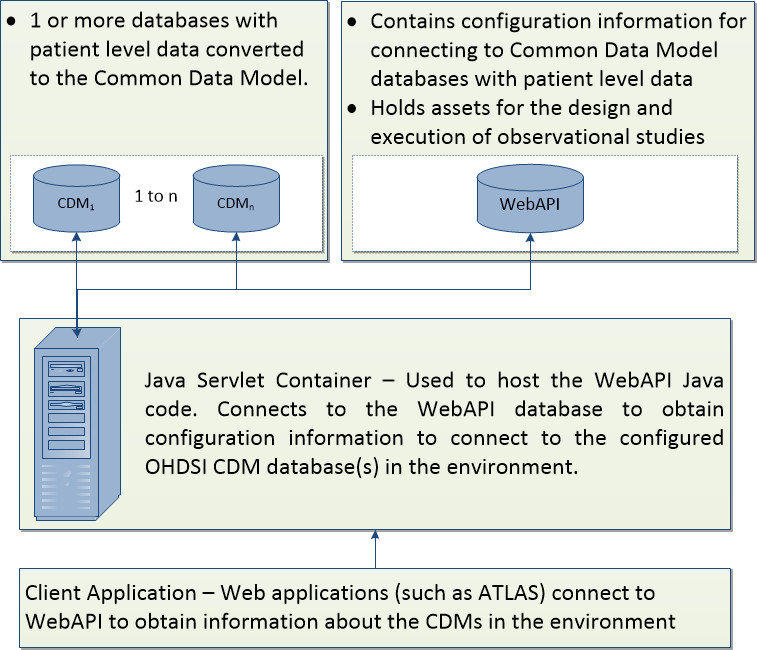
\includegraphics[width=0.50\textwidth]{figures/webAPIwiki.png}
     \caption{Estructura de la WebAPI. Extraída de \cite{githubWebAPIwiki}}.
    \label{fig:webAPIwiki}
\end{figure}

En cuanto a esta estructura es importante anotar dos observaciones cruciales para el correcto funcionamiento de la WebAPI:

\begin{enumerate}
     \item La base de datos propia de la WebAPI, que almacena toda la información relevante de su propia configuración, solo puede alojarse en una base de datos PostgreSQL. Por tanto, Broadsea solo puede desplegarse, necesariamente sobre un entorno PostgreSQL.
    \item Las bases de datos externas que se conecten a la WebAPI (véase \ref{cap:04BDEXt}), pueden alojarse en cualquier tipo de base de datos pero deben estar correctamente normalizadas al modelo común de datos (CDM) de OMOP. 

\end{enumerate}

\subsubsection{Estructura en Postgre}

Es muy importante conocer el papel de la WebAPI y su funcionamiento en PostgreSQL para el despliegue de todo el entorno de Broadsea. La documentación sobre la configuración de los esquemas de la WebAPI y el CDM puede consultarse en su repositorio de github \cite{githubCDMConfig}.

La WebAPI se implementa en Postgre a través del esquema \code{webapi}, que contiene entre otras muchas, dos tablas de especial relevancia: 

\begin{itemize}
    \item \code{sources}: Esta tabla es la que registra e integra las fuentes, es decir, las bases de datos externas, que se conectan a la WebAPI, según lo visto en la Figura \ref{fig:webAPIwiki}.
    \item \code{sources\_daimon}: Esta tabla es la que registra la estructura de esquemas de cada fuente, y garantiza que se cumpla la estructura del modelo común de datos de OMOP, según lo visto en la Figura \ref{fig:webAPIwiki}.
\end{itemize}

Opcionalmente también puede añadirse el esquema \code{temp} para permitir a la WebAPI almacenar información de forma temporal y el esquema \code{webapi\_security} si se quiere configurar el protocolo de seguridad de Broadsea (véase \ref{cap:04.2.1Seguridad}).

\subsection{El Modelo común de datos (CDM)}

\subsubsection{Estructura teórica}

La explicación en profundidad del modelo común de datos de OMOP es muy extensa y no concierne directamente a los contenidos que desarrolla este manual aunque sí es importante conocer, al menos brevemente, su estructura teórica y su implementación en Postgre. La documentación e información extensa sobre el CDM se encuentra en su repositorio de github  \cite{githubCDM}, en github pages \cite{githubPagesCDM} y en el Libro de OHDSI \cite{TheBookOfOHDSI}.

Recientemente OHDSI lanzó la sexta versión del CDM aunque aún no está totalmente integrada con todas las herramientas, por lo que el manual utiliza en la implementación de Broadsea la quinta versión del CDM. Esta versión, a modo visual, presenta la siguiente estructura:

\begin{figure}[H]
    \centering
    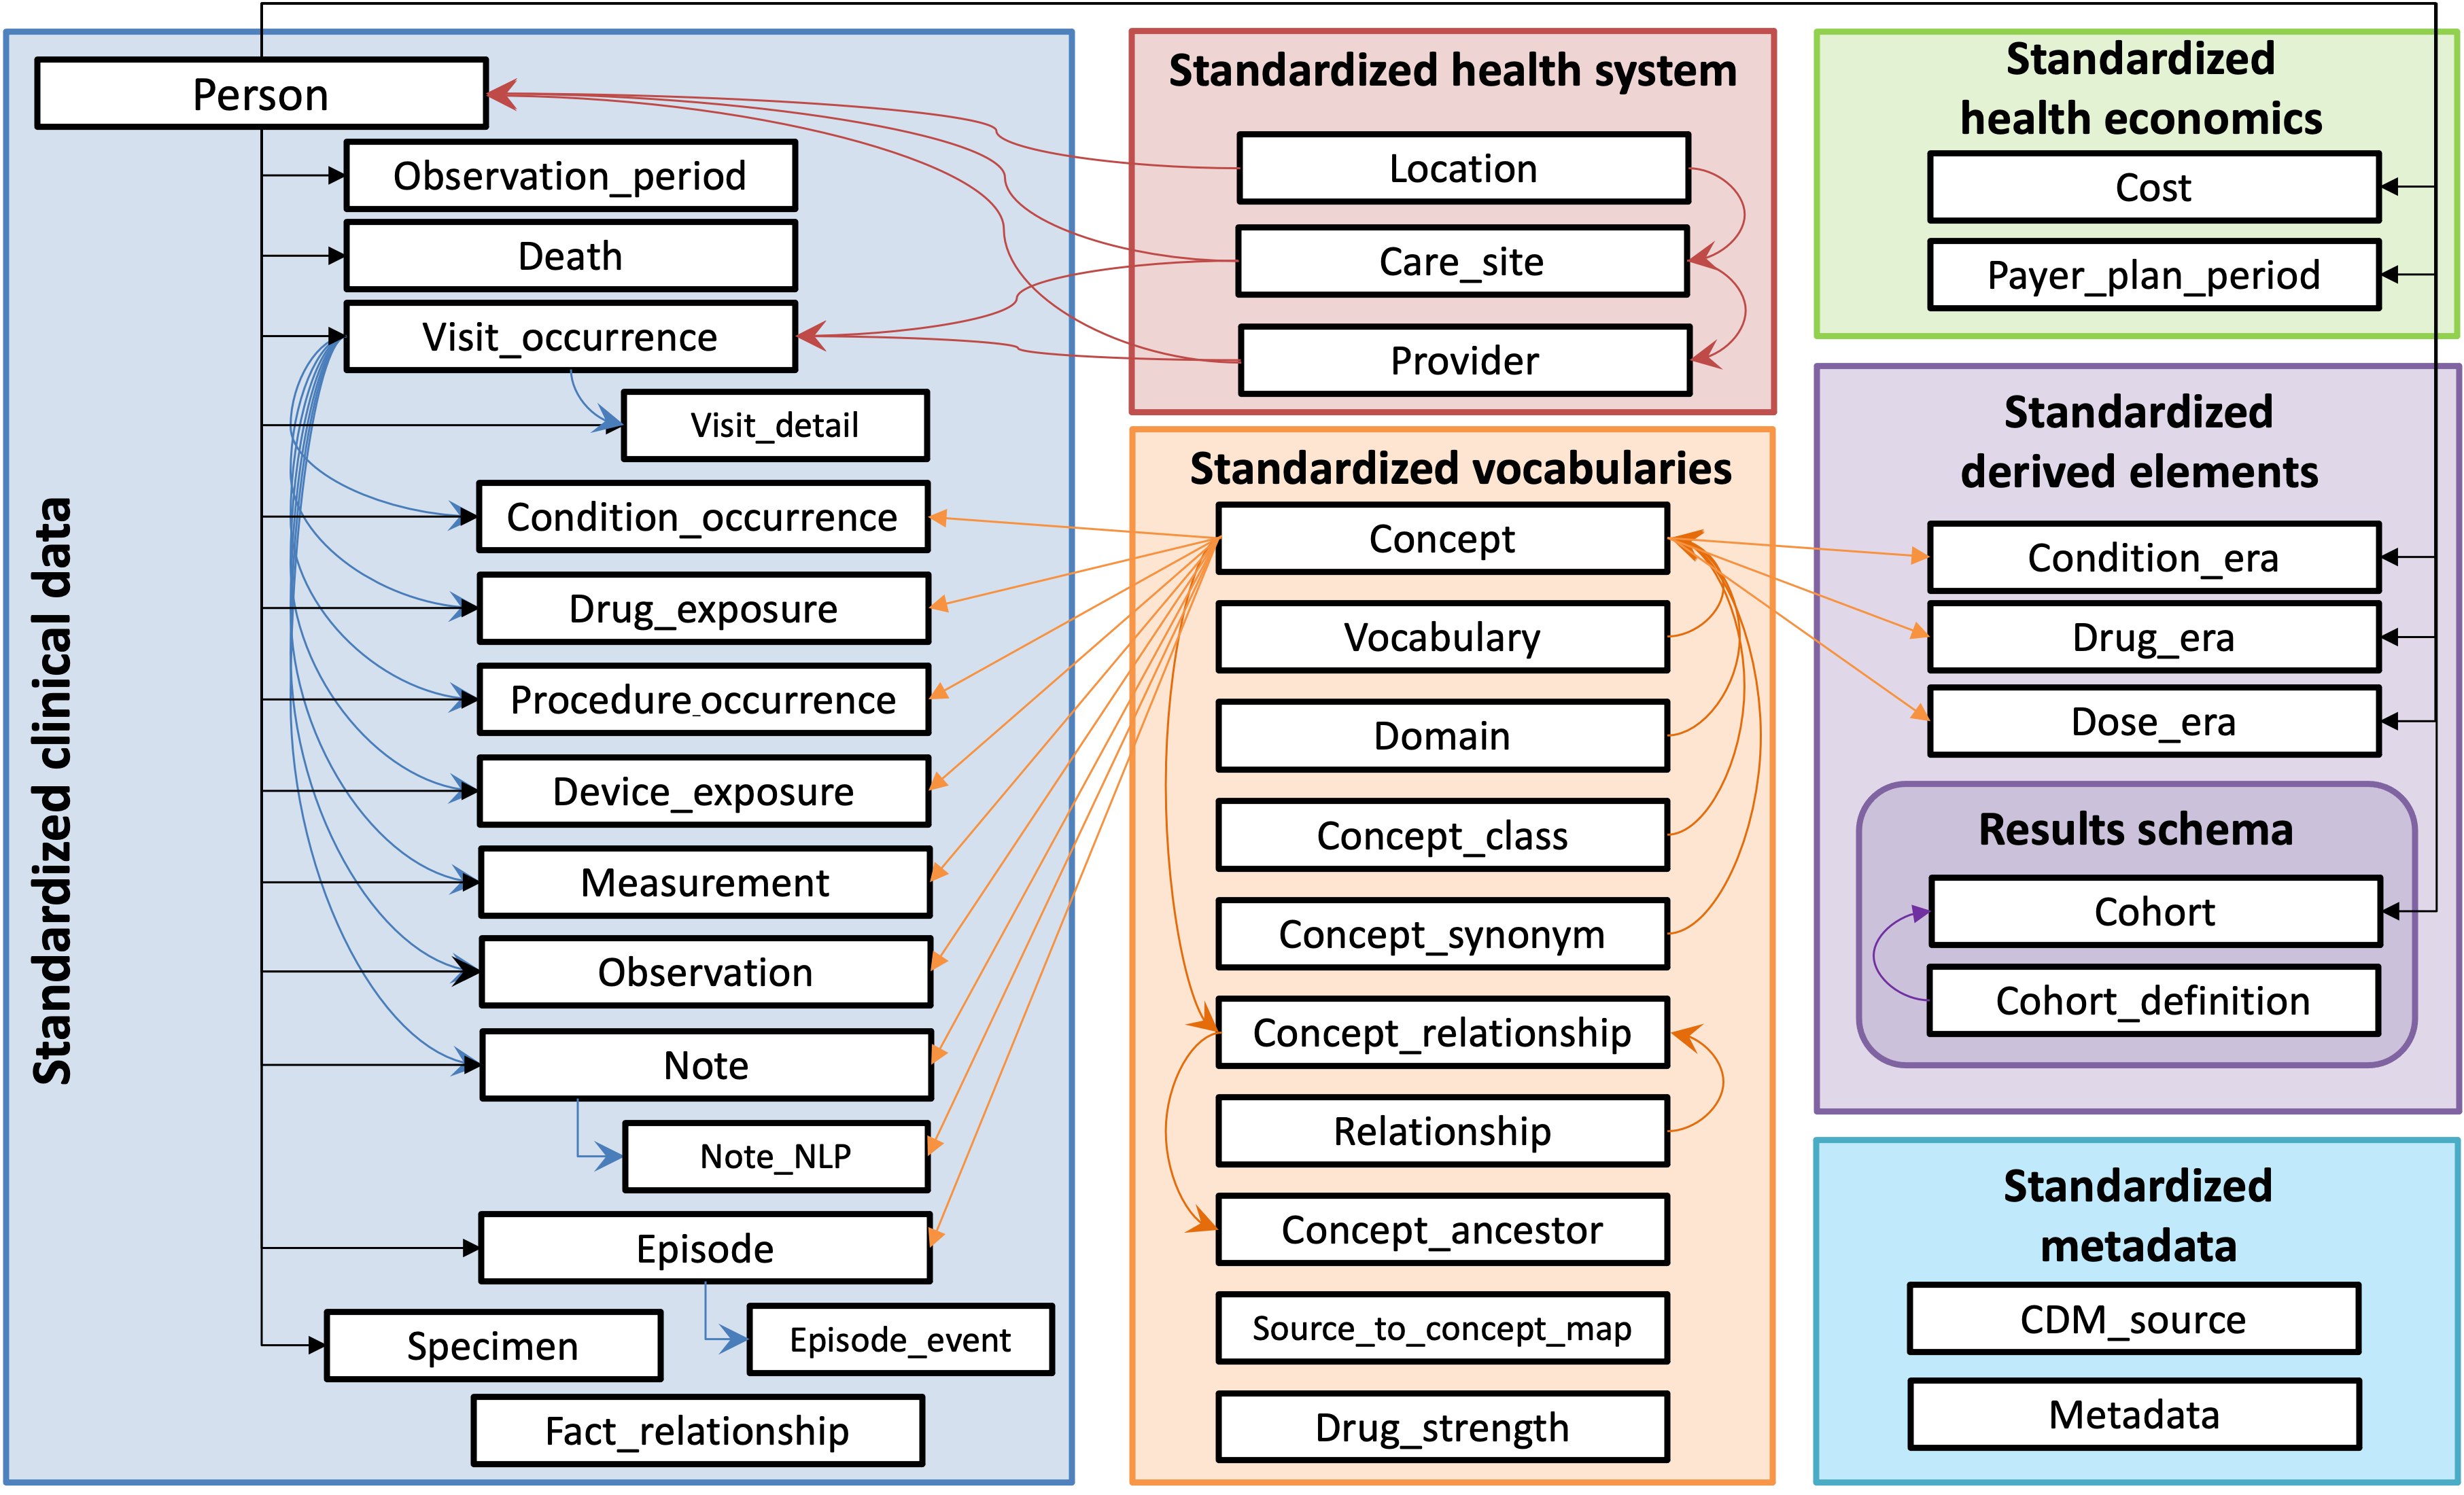
\includegraphics[width=0.80\textwidth]{figures/CDMEstructura.png}
     \caption{Estructura del CDM v5.4. Extraída de \cite{githubPagesCDM}}.
    \label{fig:CDMEstructura}
\end{figure}

Es importante, realizar una observación relevante sobre la estructura del CMD, que es la interacción entre el modelo de datos con el Vocabulario. El vocabulario se representa como una tabla más en la estructura pero es una entidad externa muy extensa y con configuración propia. La documentación sobre el Vocabulario se encuentra en la wiki de su repositorio de github \cite{githubVocabwiki} y en el Libro de OHDSI \cite{TheBookOfOHDSI}.

\subsubsection{Estructura en Postgre}

Para interactuar correctamente con Broadsea, las bases de datos externas que se integren con la WebAPI deben estar estructuradas según el CDM de OMOP. La configuración e implementación del modelo de datos se describe en su repositorio de github \cite{githubCDMConfig}. En resumen, una base de datos normalizada a OMOP debe contener al menos los siguientes esquemas:

\begin{itemize}
    \item \code{cdm}: Es el esquema que contiene todas las tablas con la información clínica de la base de datos estructurada según el CDM (véase Figura \ref{fig:CDMEstructura}). Su presencia es obligatoria.
    \item \code{results}: Es el esquema donde se almacenan los resultados obtenidos tras los análisis que realiza la herramienta. Se separa del \code{cdm} para evitar mezclar la información de la base de datos de solo lectura y la información producida por el usuario. Su presencia es obligatoria.
    \item \code{vocab}: Es el esquema donde se almacena el Vocabulario. Su configuración es obligatoria aunque puede aparecer implícito en el \code{cdm} o como un esquema externo. Si hay varias bases de datos que utilicen el mismo Vocabulario no es necesario configurar un Vocabulario para cada una, basta con que se implemente uno y el resto apunten a él.
\end{itemize}

\subsection{Estructura de Broadsea}

Por último, presentar concretamente la estructura que adopta Broadsea al desplegarse en Postgre. Pues si bien Broadsea se virtualiza gracias a Docker, se puede acceder a su base de datos de forma local gracias a la conexión con el servidor Postgre de Broadsea. La información relevante a la base de datos de Broadsea se puede consultar en su repositorio de github \cite{githubBroadseaDB}.

En su configuración por defecto (véase \ref{cap:03ConexLocal}), el servidor de Broadsea se configura en el localhost (bien en el 0.0.0.0  o en 127.0.0.1), en el puerto 5432 \cite{githubBroadseaDB} y alberga una única base de datos en la que combina la información de la WebAPI y una pequeña muestra de la base de datos de Eunomia. Para acceder a la documentación sobre Eunomia se consultar su repositorio de github \cite{githubEunomia} o github pages \cite{githubPagesEunomia}.

Es decir, la base de datos inicial de Broadsea presenta cinco esquemas:

\begin{itemize}
    \item \code{public}: Es el esquema por defecto que se crea con cualquier base de datos Postgre.
    \item \code{webapi}: Corresponde al esquema \code{webapi} de la estructura de la WebAPI. Presenta la información de configuración del entorno.
    \item \code{webapi\_security}: Es un esquema opcional para activar la seguridad de la WebAPI y ATLAS. No se utiliza en el manual.
    \item \code{demo\_cdm}: Corresponde al esquema \code{cdm} de la estructura del CDM. Alberga el contenido de la base de datos de Eunomia y una pequeña muestra implícita del Vocabulario.
    \item \code{demo\_cdm\_results}:  Es el esquema que corresponde al esquema \code{results} de la estructura del CDM.
\end{itemize}

Es importante anotar que la configuración por defecto de Broadsea trae una pequeña muestra del Vocabulario pero muy insignificante, por lo que para realizar análisis en profundidad será necesario configurar un esquema que albergue información más extensa (véase \ref{cap:05Vocab}).

\section{Recapitulación}

A esta altura, queda recogido en \ref{cap:01.1IntroManual} la introducción al manual, el motivo por el que se redacta, la necesidad que subyace al mismo y el contexto en el que se realiza la instalación y  en \ref{cap:01.2descripBroadsea}, \ref{cap:01.3Docker}, \ref{01.4Postgre}, la descripción teórica de Broadsea y el desglose en las distintas herramientas que permiten su despliegue.

Por tanto, a partir de este momento comienza en \ref{cap:02Despliegue}, \ref{cap:03ConexLocal}, \ref{cap:04BDEXt} y \ref{cap:05Vocab} la implementación práctica de todos los contenidos presentados, orientados específicamente a la instalación y configuración de la herramienta ATLAS. 

En conclusión, si bien hasta ahora se presentaba Broadsea de forma general, el enfoque de las sigueintes secciones gira concretamente entorno a ATLAS Broadsea.



